\documentclass[]{article}
\usepackage{lmodern}
\usepackage{amssymb,amsmath}
\usepackage{ifxetex,ifluatex}
\usepackage{fixltx2e} % provides \textsubscript
\ifnum 0\ifxetex 1\fi\ifluatex 1\fi=0 % if pdftex
  \usepackage[T1]{fontenc}
  \usepackage[utf8]{inputenc}
\else % if luatex or xelatex
  \ifxetex
    \usepackage{mathspec}
    \usepackage{xltxtra,xunicode}
  \else
    \usepackage{fontspec}
  \fi
  \defaultfontfeatures{Mapping=tex-text,Scale=MatchLowercase}
  \newcommand{\euro}{€}
\fi
% use upquote if available, for straight quotes in verbatim environments
\IfFileExists{upquote.sty}{\usepackage{upquote}}{}
% use microtype if available
\IfFileExists{microtype.sty}{%
\usepackage{microtype}
\UseMicrotypeSet[protrusion]{basicmath} % disable protrusion for tt fonts
}{}
\usepackage[margin=1in]{geometry}
\usepackage{color}
\usepackage{fancyvrb}
\newcommand{\VerbBar}{|}
\newcommand{\VERB}{\Verb[commandchars=\\\{\}]}
\DefineVerbatimEnvironment{Highlighting}{Verbatim}{commandchars=\\\{\}}
% Add ',fontsize=\small' for more characters per line
\usepackage{framed}
\definecolor{shadecolor}{RGB}{248,248,248}
\newenvironment{Shaded}{\begin{snugshade}}{\end{snugshade}}
\newcommand{\KeywordTok}[1]{\textcolor[rgb]{0.13,0.29,0.53}{\textbf{{#1}}}}
\newcommand{\DataTypeTok}[1]{\textcolor[rgb]{0.13,0.29,0.53}{{#1}}}
\newcommand{\DecValTok}[1]{\textcolor[rgb]{0.00,0.00,0.81}{{#1}}}
\newcommand{\BaseNTok}[1]{\textcolor[rgb]{0.00,0.00,0.81}{{#1}}}
\newcommand{\FloatTok}[1]{\textcolor[rgb]{0.00,0.00,0.81}{{#1}}}
\newcommand{\CharTok}[1]{\textcolor[rgb]{0.31,0.60,0.02}{{#1}}}
\newcommand{\StringTok}[1]{\textcolor[rgb]{0.31,0.60,0.02}{{#1}}}
\newcommand{\CommentTok}[1]{\textcolor[rgb]{0.56,0.35,0.01}{\textit{{#1}}}}
\newcommand{\OtherTok}[1]{\textcolor[rgb]{0.56,0.35,0.01}{{#1}}}
\newcommand{\AlertTok}[1]{\textcolor[rgb]{0.94,0.16,0.16}{{#1}}}
\newcommand{\FunctionTok}[1]{\textcolor[rgb]{0.00,0.00,0.00}{{#1}}}
\newcommand{\RegionMarkerTok}[1]{{#1}}
\newcommand{\ErrorTok}[1]{\textbf{{#1}}}
\newcommand{\NormalTok}[1]{{#1}}
\usepackage{graphicx}
\makeatletter
\def\maxwidth{\ifdim\Gin@nat@width>\linewidth\linewidth\else\Gin@nat@width\fi}
\def\maxheight{\ifdim\Gin@nat@height>\textheight\textheight\else\Gin@nat@height\fi}
\makeatother
% Scale images if necessary, so that they will not overflow the page
% margins by default, and it is still possible to overwrite the defaults
% using explicit options in \includegraphics[width, height, ...]{}
\setkeys{Gin}{width=\maxwidth,height=\maxheight,keepaspectratio}
\ifxetex
  \usepackage[setpagesize=false, % page size defined by xetex
              unicode=false, % unicode breaks when used with xetex
              xetex]{hyperref}
\else
  \usepackage[unicode=true]{hyperref}
\fi
\hypersetup{breaklinks=true,
            bookmarks=true,
            pdfauthor={JcB},
            pdftitle={Analyse le fichier mergé},
            colorlinks=true,
            citecolor=blue,
            urlcolor=blue,
            linkcolor=magenta,
            pdfborder={0 0 0}}
\urlstyle{same}  % don't use monospace font for urls
\setlength{\parindent}{0pt}
\setlength{\parskip}{6pt plus 2pt minus 1pt}
\setlength{\emergencystretch}{3em}  % prevent overfull lines
\setcounter{secnumdepth}{5}

%%% Use protect on footnotes to avoid problems with footnotes in titles
\let\rmarkdownfootnote\footnote%
\def\footnote{\protect\rmarkdownfootnote}

%%% Change title format to be more compact
\usepackage{titling}

% Create subtitle command for use in maketitle
\newcommand{\subtitle}[1]{
  \posttitle{
    \begin{center}\large#1\end{center}
    }
}

\setlength{\droptitle}{-2em}
  \title{Analyse le fichier mergé}
  \pretitle{\vspace{\droptitle}\centering\huge}
  \posttitle{\par}
  \author{JcB}
  \preauthor{\centering\large\emph}
  \postauthor{\par}
  \predate{\centering\large\emph}
  \postdate{\par}
  \date{22/11/2015}



\begin{document}

\maketitle


{
\hypersetup{linkcolor=black}
\setcounter{tocdepth}{2}
\tableofcontents
}
Alalyse le fichier \textbf{merge2015} résultant du merging des fichiers
\textbf{dpr2} et \textbf{orumip}. Voir README.md pour la signification
des fichiers. Le fichier \emph{merge2015} est par
\textbf{Analyse\_regroupement}.

\section{Récupération des fichiers de
travail}\label{recuperation-des-fichiers-de-travail}

\begin{Shaded}
\begin{Highlighting}[]
\KeywordTok{library}\NormalTok{(epicalc)}
\end{Highlighting}
\end{Shaded}

\begin{verbatim}
## Loading required package: foreign
## Loading required package: survival
## Loading required package: MASS
## Loading required package: nnet
\end{verbatim}

\begin{Shaded}
\begin{Highlighting}[]
\NormalTok{path <-}\StringTok{ "../"} \CommentTok{# path <- "" en mode console}

\KeywordTok{load}\NormalTok{(}\StringTok{"../Regroupement_ORUMIP/merge2015.Rda"}\NormalTok{) }\CommentTok{# le fichier mergé}
\KeywordTok{source}\NormalTok{(}\KeywordTok{paste0}\NormalTok{(path,}\StringTok{"regroupement.R"}\NormalTok{))}

\NormalTok{d3 <-}\StringTok{ }\NormalTok{merge2015 }\CommentTok{# pour rendre le programme générique}
\NormalTok{anc <-}\StringTok{ }\DecValTok{2015}

\KeywordTok{names}\NormalTok{(d3)}
\end{Highlighting}
\end{Shaded}

\begin{verbatim}
##  [1] "DP"            "id"            "CODE_POSTAL"   "COMMUNE"      
##  [5] "DESTINATION"   "ENTREE"        "EXTRACT"       "FINESS"       
##  [9] "GRAVITE"       "MODE_ENTREE"   "MODE_SORTIE"   "MOTIF"        
## [13] "NAISSANCE"     "ORIENTATION"   "PROVENANCE"    "SEXE"         
## [17] "SORTIE"        "TRANSPORT"     "TRANSPORT_PEC" "AGE"          
## [21] "LIBELLE_CIM10" "SFMU"          "TYPE_URGENCES" "CHAPITRE"     
## [25] "SOUS_CHAPITRE"
\end{verbatim}

\begin{Shaded}
\begin{Highlighting}[]
\KeywordTok{summary}\NormalTok{(d3$TYPE_URGENCES)}
\end{Highlighting}
\end{Shaded}

\begin{verbatim}
##      Autre recours Médico-chirurgical      Psychiatrique 
##               8145             147819               5677 
##      Toxicologique    Traumatologique               NA's 
##               4180              99558                296
\end{verbatim}

\begin{Shaded}
\begin{Highlighting}[]
\CommentTok{# Décommenter si nécessaire. Affichage volumineux}
\CommentTok{# summary(d3$CHAPITRE)}
\CommentTok{# summary(d3$SOUS_CHAPITRE)}

\KeywordTok{tapply}\NormalTok{(d3$TYPE_URGENCES, }\KeywordTok{list}\NormalTok{(d3$FINESS, d3$TYPE_URGENCES), length)}
\end{Highlighting}
\end{Shaded}

\begin{verbatim}
##     Autre recours Médico-chirurgical Psychiatrique Toxicologique
## 3Fr           514               4684           152            68
## Alk           163               1134            49            16
## Ane            NA                 NA            NA            NA
## Col          2243              25717          1367           915
## Dia           489               5923           109             3
## Dts            NA               1618            NA            NA
## Geb           530               6062           122           111
## Hag           738              17936           461           468
## Hus            NA                 NA            NA            NA
## Mul          1056              18671          1416           696
## Odi            97               6833            55             2
## Ros            NA                 NA            NA            NA
## Sav           149               2640           133            76
## Sel           785              11274           242           355
## Wis           409               5398           207            94
## HTP           450              22884           506           493
## NHC           138              10008           268           564
## Emr           324               4812           565           286
## Hsr            60               2225            25            33
## Ccm            NA                 NA            NA            NA
##     Traumatologique
## 3Fr            3525
## Alk            1315
## Ane              NA
## Col           19205
## Dia            4012
## Dts            6080
## Geb            6659
## Hag           10948
## Hus              NA
## Mul            7819
## Odi            3048
## Ros             502
## Sav            2724
## Sel           10863
## Wis            3901
## HTP           15133
## NHC             602
## Emr            3215
## Hsr               7
## Ccm              NA
\end{verbatim}

\subsection{Type d'urgence}\label{type-durgence}

\begin{Shaded}
\begin{Highlighting}[]
\NormalTok{n.type <-}\StringTok{ }\KeywordTok{nrow}\NormalTok{(d3)}
\NormalTok{s.type <-}\StringTok{ }\KeywordTok{summary}\NormalTok{(d3$TYPE_URGENCES)}
\NormalTok{s.type}
\end{Highlighting}
\end{Shaded}

\begin{verbatim}
##      Autre recours Médico-chirurgical      Psychiatrique 
##               8145             147819               5677 
##      Toxicologique    Traumatologique               NA's 
##               4180              99558                296
\end{verbatim}

\begin{Shaded}
\begin{Highlighting}[]
\KeywordTok{pie}\NormalTok{(s.type, }\DataTypeTok{main =} \KeywordTok{paste0}\NormalTok{(anc, }\StringTok{" - Grands groupes diagnostics"}\NormalTok{), }\DataTypeTok{col =} \KeywordTok{c}\NormalTok{(}\StringTok{"yellow"}\NormalTok{,}\StringTok{"blue"}\NormalTok{, }\StringTok{"orange"}\NormalTok{, }\StringTok{"green"}\NormalTok{, }\StringTok{"red"}\NormalTok{,}\StringTok{"black"}\NormalTok{))}
\end{Highlighting}
\end{Shaded}

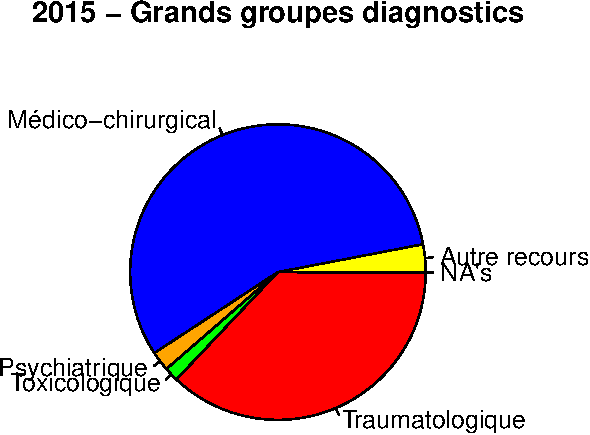
\includegraphics{analyse_merge_files/figure-latex/type_urgence-1.pdf}

\begin{Shaded}
\begin{Highlighting}[]
\KeywordTok{par}\NormalTok{(}\DataTypeTok{mar =} \KeywordTok{c}\NormalTok{(}\DecValTok{6}\NormalTok{,}\DecValTok{4}\NormalTok{,}\DecValTok{3}\NormalTok{,}\DecValTok{2}\NormalTok{))}
\KeywordTok{barplot}\NormalTok{(}\KeywordTok{sort}\NormalTok{(s.type, }\DataTypeTok{decreasing =} \OtherTok{TRUE}\NormalTok{), }\DataTypeTok{las =} \DecValTok{2}\NormalTok{, }\DataTypeTok{cex.names =} \FloatTok{0.7}\NormalTok{, }\DataTypeTok{main =} \StringTok{"Répartition des diagnostics principaux }\CharTok{\textbackslash{}n}\StringTok{selon les codes de regroupement de l' ORUMIP"}\NormalTok{)}
\end{Highlighting}
\end{Shaded}

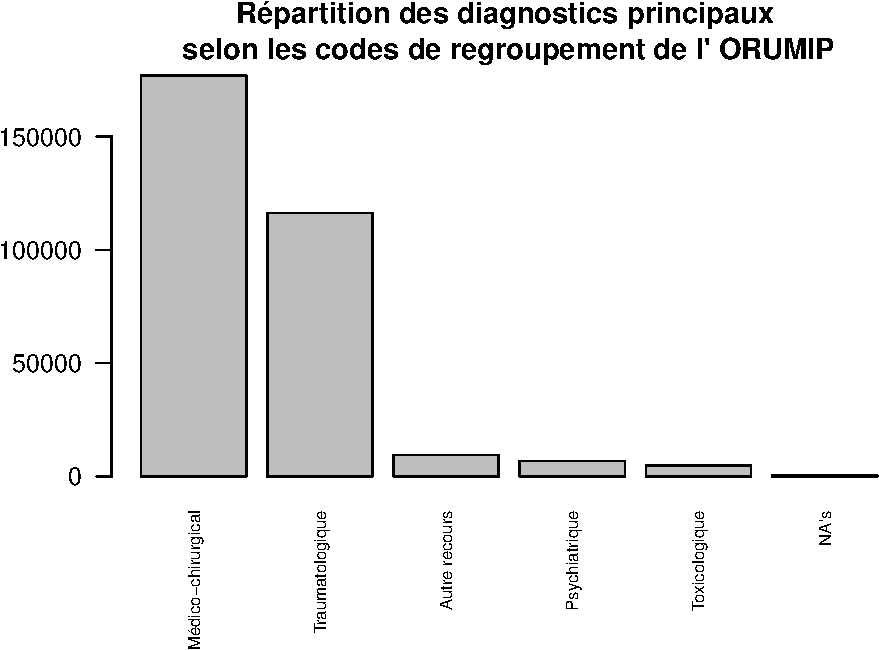
\includegraphics{analyse_merge_files/figure-latex/type_urgence-2.pdf}

\begin{Shaded}
\begin{Highlighting}[]
\KeywordTok{tab1}\NormalTok{(d3$TYPE_URGENCES, }\DataTypeTok{sort.group =} \StringTok{"decreasing"}\NormalTok{, }\DataTypeTok{cex.names =} \FloatTok{0.6}\NormalTok{, }\DataTypeTok{main =} \StringTok{"Répartition des diagnostics principaux }\CharTok{\textbackslash{}n}\StringTok{selon les codes de regroupement de l' ORUMIP"}\NormalTok{)}
\end{Highlighting}
\end{Shaded}

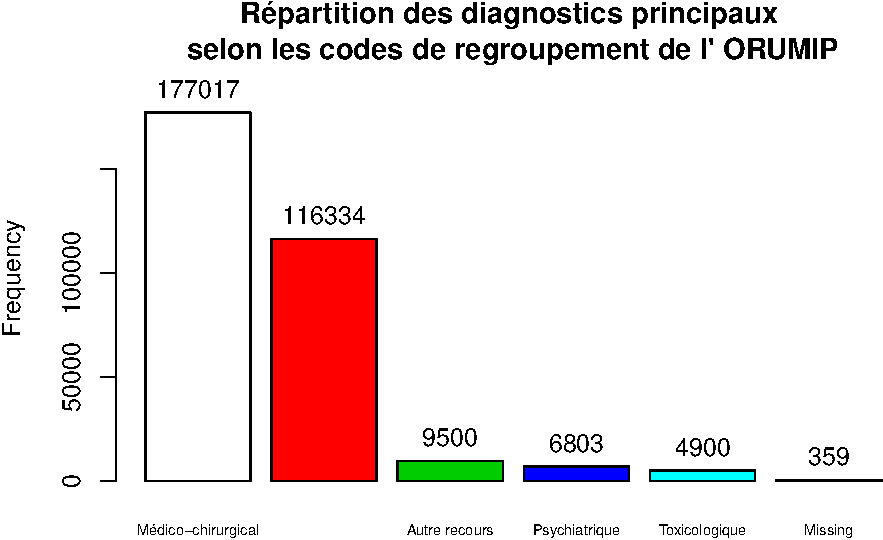
\includegraphics{analyse_merge_files/figure-latex/type_urgence-3.pdf}

\begin{verbatim}
## d3$TYPE_URGENCES : 
##                    Frequency   %(NA+)   %(NA-)
## Médico-chirurgical    147819     55.6     55.7
## Traumatologique        99558     37.5     37.5
## Autre recours           8145      3.1      3.1
## Psychiatrique           5677      2.1      2.1
## Toxicologique           4180      1.6      1.6
## NA's                     296      0.1      0.0
##   Total               265675    100.0    100.0
\end{verbatim}

296 codes de sont pas reconnus
(\texttt{s.type{[}"NA\textquotesingle{}s"{]}*100/n.type} \%).

\begin{Shaded}
\begin{Highlighting}[]
\NormalTok{a <-}\StringTok{ }\NormalTok{d3[}\KeywordTok{is.na}\NormalTok{(d3$TYPE_URGENCES),]}
\KeywordTok{cbind}\NormalTok{(}\KeywordTok{summary}\NormalTok{(}\KeywordTok{as.factor}\NormalTok{(a$DP)))}
\end{Highlighting}
\end{Shaded}

\begin{verbatim}
##                     [,1]
## I200+                 11
## N23 0                 10
## W5700                  9
## W0689                  6
## V4259                  5
## W5701                  5
## X6591                  5
## W1008                  4
## Y1509                  4
## M459                   3
## T16 0                  3
## V1938                  3
## V4269                  3
## W5709                  3
## W5781                  3
## W5799                  3
## Y3343                  3
## S011 02                2
## S2250+B6               2
## V1328                  2
## V4859                  2
## W0184                  2
## W0694                  2
## W0704                  2
## W0709                  2
## W1959                  2
## W4483                  2
## W4581                  2
## W5434                  2
## W5703                  2
## W5704                  2
## W5743                  2
## X2302                  2
## X4548                  2
## X4594                  2
## X6102                  2
## X6434                  2
## Y1559                  2
## Y3341                  2
## F034                   1
## G510 02                1
## GH819) VERTIGES        1
## J90 0                  1
## JJ189) PNEUMOPATHIE    1
## K409 01                1
## MM199) ARTHROSE SP     1
## MM255) ARTHRALGIES     1
## S202 02                1
## S223 01                1
## S372(0                 1
## S422 02                1
## S720 02                1
## S729 01                1
## S800 01                1
## S801 02                1
## S823 01                1
## S929 01                1
## SS331                  1
## SV899) AVP             1
## SY099) AGRESSION       1
## U152                   1
## V0408                  1
## V1293                  1
## V1931                  1
## V2658                  1
## V4008                  1
## V4053                  1
## V4202                  1
## V4654                  1
## V5201                  1
## V5351                  1
## V7894                  1
## V9312                  1
## W0104                  1
## W0123                  1
## W0458                  1
## W0604                  1
## W0609                  1
## W0620                  1
## W1048                  1
## W1100                  1
## W1323                  1
## W1378                  1
## W1721                  1
## W1739                  1
## W1788                  1
## W1791                  1
## W1849                  1
## W1904                  1
## W1910                  1
## W1929                  1
## W1949                  1
## W1950                  1
## W1981                  1
## W1989                  1
## W1998                  1
## W1999                  1
## W4402                  1
## W4403                  1
## (Other)              109
\end{verbatim}

\begin{itemize}
\itemsep1pt\parskip0pt\parsep0pt
\item
  Plus de la moitié des codes concernent \textbf{R53+0}, \textbf{R53+1}
  et \textbf{R53+2} qui sont des codes PMSI. \emph{R53} = Malaise et
  fatigue.
\item
  r11 = vomissements: pb de casse
\item
  B99+1 = Syndrome infectieux sans cause trouvée
\end{itemize}

exemple pour Mulhouse:

\begin{Shaded}
\begin{Highlighting}[]
\NormalTok{mul <-}\StringTok{ }\NormalTok{merge2015[}\KeywordTok{is.na}\NormalTok{(merge2015$LIBELLE_CIM10) &}\StringTok{ }\NormalTok{merge2015$FINESS %in%}\StringTok{ }\KeywordTok{c}\NormalTok{(}\StringTok{"Mul"}\NormalTok{,}\StringTok{"Hsr"}\NormalTok{,}\StringTok{"Emr"}\NormalTok{),]}
\NormalTok{mulx <-}\StringTok{ }\KeywordTok{cbind}\NormalTok{(}\KeywordTok{summary}\NormalTok{(}\KeywordTok{as.factor}\NormalTok{(mul$DP)))}
\NormalTok{mulx}
\end{Highlighting}
\end{Shaded}

\begin{verbatim}
##                     [,1]
## GH819) VERTIGES        1
## JJ189) PNEUMOPATHIE    1
## M459                   3
## MM199) ARTHROSE SP     1
## MM255) ARTHRALGIES     1
## S2250+B6               2
## S372(0                 1
## SV899) AVP             1
## SY099) AGRESSION       1
## Z                      1
\end{verbatim}

\section{Par type d'urgence}\label{par-type-durgence}

Le regroupement principal de l'ORUMIP comprend les chapitres suivants:

\begin{verbatim}
[1] "Autre recours"      "Médico-chirurgical" "Psychiatrique"     
[4] "Toxicologique"      "Traumatologique"   
\end{verbatim}

\subsection{Analyse des urgences
médico-chirurgicales}\label{analyse-des-urgences-medico-chirurgicales}

\begin{Shaded}
\begin{Highlighting}[]
\NormalTok{s.type <-}\StringTok{ }\KeywordTok{summary}\NormalTok{(d3$TYPE_URGENCES)}
\KeywordTok{sort}\NormalTok{(s.type, }\DataTypeTok{decreasing =} \OtherTok{TRUE}\NormalTok{)}
\end{Highlighting}
\end{Shaded}

\begin{verbatim}
## Médico-chirurgical    Traumatologique      Autre recours 
##             147819              99558               8145 
##      Psychiatrique      Toxicologique               NA's 
##               5677               4180                296
\end{verbatim}

\begin{Shaded}
\begin{Highlighting}[]
\NormalTok{medic <-}\StringTok{ }\NormalTok{d3[d3$TYPE_URGENCES ==}\StringTok{ "Médico-chirurgical"}\NormalTok{,]}

\KeywordTok{tab1}\NormalTok{(}\KeywordTok{factor}\NormalTok{(medic$CHAPITRE), }\DataTypeTok{sort.group =} \StringTok{"decreasing"}\NormalTok{, }\DataTypeTok{bar.values =} \StringTok{"percent"}\NormalTok{, }\DataTypeTok{cex.names =} \FloatTok{0.8}\NormalTok{, }\DataTypeTok{main =} \StringTok{"Médico-chirurgical"}\NormalTok{)}
\end{Highlighting}
\end{Shaded}

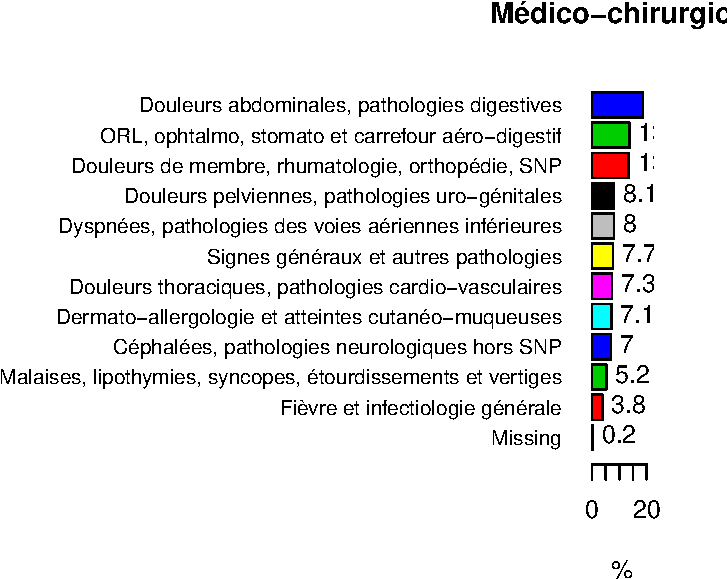
\includegraphics{analyse_merge_files/figure-latex/chapitre-1.pdf}

\begin{verbatim}
## factor(medic$CHAPITRE) : 
##                                                              Frequency
## Douleurs abdominales, pathologies digestives                     27580
## ORL, ophtalmo, stomato et carrefour aéro-digestif                20334
## Douleurs de membre, rhumatologie, orthopédie, SNP                19834
## Douleurs pelviennes, pathologies uro-génitales                   11930
## Dyspnées, pathologies des voies aériennes inférieures            11820
## Signes généraux et autres pathologies                            11363
## Douleurs thoraciques, pathologies cardio-vasculaires             10858
## Dermato-allergologie et atteintes cutanéo-muqueuses              10464
## Céphalées, pathologies neurologiques hors SNP                    10302
## Malaises, lipothymies, syncopes, étourdissements et vertiges      7632
## Fièvre et infectiologie générale                                  5702
## NA's                                                               296
##   Total                                                         148115
##                                                                %(NA+)
## Douleurs abdominales, pathologies digestives                     18.6
## ORL, ophtalmo, stomato et carrefour aéro-digestif                13.7
## Douleurs de membre, rhumatologie, orthopédie, SNP                13.4
## Douleurs pelviennes, pathologies uro-génitales                    8.1
## Dyspnées, pathologies des voies aériennes inférieures             8.0
## Signes généraux et autres pathologies                             7.7
## Douleurs thoraciques, pathologies cardio-vasculaires              7.3
## Dermato-allergologie et atteintes cutanéo-muqueuses               7.1
## Céphalées, pathologies neurologiques hors SNP                     7.0
## Malaises, lipothymies, syncopes, étourdissements et vertiges      5.2
## Fièvre et infectiologie générale                                  3.8
## NA's                                                              0.2
##   Total                                                         100.0
##                                                                %(NA-)
## Douleurs abdominales, pathologies digestives                     18.7
## ORL, ophtalmo, stomato et carrefour aéro-digestif                13.8
## Douleurs de membre, rhumatologie, orthopédie, SNP                13.4
## Douleurs pelviennes, pathologies uro-génitales                    8.1
## Dyspnées, pathologies des voies aériennes inférieures             8.0
## Signes généraux et autres pathologies                             7.7
## Douleurs thoraciques, pathologies cardio-vasculaires              7.3
## Dermato-allergologie et atteintes cutanéo-muqueuses               7.1
## Céphalées, pathologies neurologiques hors SNP                     7.0
## Malaises, lipothymies, syncopes, étourdissements et vertiges      5.2
## Fièvre et infectiologie générale                                  3.9
## NA's                                                              0.0
##   Total                                                         100.0
\end{verbatim}

\subsection{Analyse des urgences
médico-chirurgicales}\label{analyse-des-urgences-medico-chirurgicales-1}

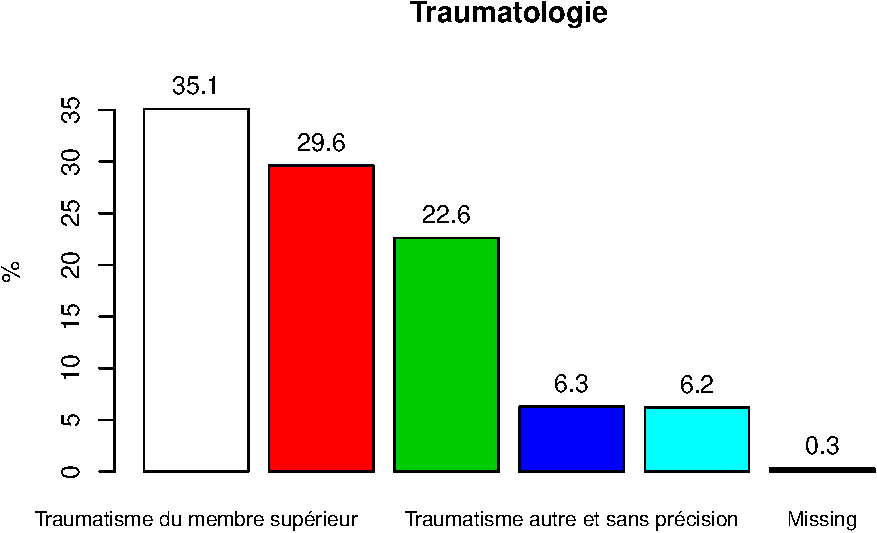
\includegraphics{analyse_merge_files/figure-latex/urg_traumato-1.pdf}

\begin{verbatim}
## factor(trauma$CHAPITRE) : 
##                                      Frequency   %(NA+)   %(NA-)
## Traumatisme du membre supérieur          35340     35.4     35.5
## Traumatisme du membre inférieur          29599     29.6     29.7
## Traumatisme de la tête et du cou         22271     22.3     22.4
## Traumatisme autre et sans précision       6254      6.3      6.3
## Traumatisme thoraco-abdomino-pelvien      6094      6.1      6.1
## NA's                                       296      0.3      0.0
##   Total                                  99854    100.0    100.0
\end{verbatim}

\section{Par age}\label{par-age}

\subsection{Adultes (18 à 75 ans)}\label{adultes-18-a-75-ans}

\begin{Shaded}
\begin{Highlighting}[]
\NormalTok{d3a <-}\StringTok{ }\NormalTok{d3[d3$AGE >}\StringTok{ }\DecValTok{17} \NormalTok{&}\StringTok{ }\NormalTok{d3$AGE <}\StringTok{ }\DecValTok{76}\NormalTok{,]}
\NormalTok{n.adl <-}\StringTok{ }\KeywordTok{nrow}\NormalTok{(d3a)}

\CommentTok{# table fréquence}
\NormalTok{s.type.adl <-}\StringTok{ }\KeywordTok{table}\NormalTok{(d3a$TYPE_URGENCES)}
\NormalTok{s.type.adl}
\end{Highlighting}
\end{Shaded}

\begin{verbatim}
## 
##      Autre recours Médico-chirurgical      Psychiatrique 
##               5375              80448               4532 
##      Toxicologique    Traumatologique 
##               3546              53216
\end{verbatim}

\begin{Shaded}
\begin{Highlighting}[]
\CommentTok{# table des proportion}
\NormalTok{p.type.adl <-}\StringTok{ }\KeywordTok{round}\NormalTok{(}\KeywordTok{prop.table}\NormalTok{(s.type.adl) *}\StringTok{ }\DecValTok{100}\NormalTok{, }\DecValTok{2}\NormalTok{)}
\NormalTok{p.type.adl}
\end{Highlighting}
\end{Shaded}

\begin{verbatim}
## 
##      Autre recours Médico-chirurgical      Psychiatrique 
##               3.65              54.68               3.08 
##      Toxicologique    Traumatologique 
##               2.41              36.17
\end{verbatim}

\begin{Shaded}
\begin{Highlighting}[]
\KeywordTok{pie}\NormalTok{(s.type.adl, }\DataTypeTok{main =} \StringTok{"Adultes"}\NormalTok{, }\DataTypeTok{cex=}\FloatTok{0.8}\NormalTok{, }\DataTypeTok{col =} \KeywordTok{palette}\NormalTok{(}\KeywordTok{heat.colors}\NormalTok{(}\DecValTok{6}\NormalTok{)))}
\end{Highlighting}
\end{Shaded}

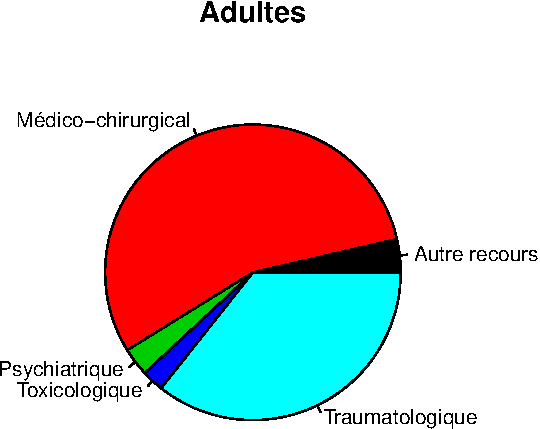
\includegraphics{analyse_merge_files/figure-latex/adultes-1.pdf}

\begin{Shaded}
\begin{Highlighting}[]
\NormalTok{taba <-}\StringTok{ }\KeywordTok{tab1}\NormalTok{(d3a$TYPE_URGENCES, }\DataTypeTok{sort.group =} \StringTok{"decreasing"}\NormalTok{, }\DataTypeTok{bar.values =} \StringTok{"percent"}\NormalTok{, }\DataTypeTok{cex.names =} \FloatTok{0.8}\NormalTok{, }\DataTypeTok{main =} \KeywordTok{paste0}\NormalTok{(}\StringTok{"Médico-chirurgical adulte (N = "}\NormalTok{, n.adl, }\StringTok{")"}\NormalTok{), }\DataTypeTok{missing =} \OtherTok{FALSE}\NormalTok{)}
\end{Highlighting}
\end{Shaded}

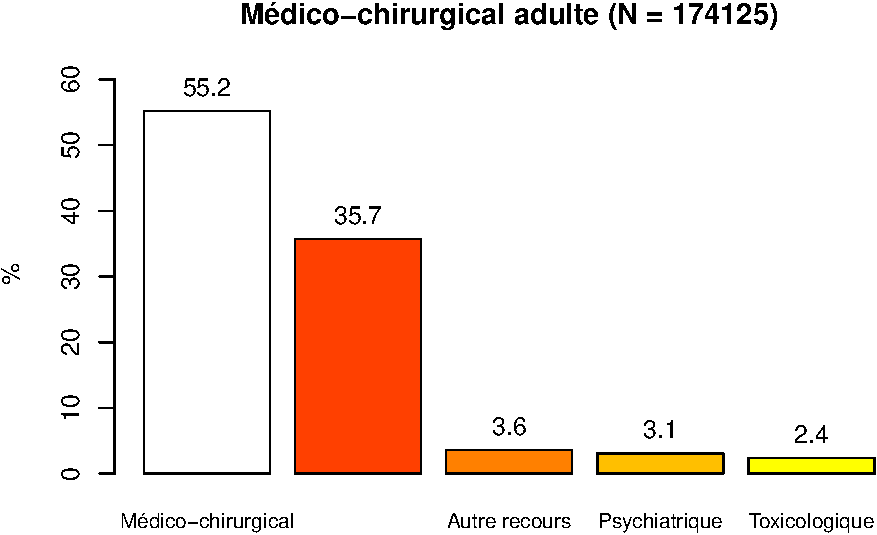
\includegraphics{analyse_merge_files/figure-latex/adultes-2.pdf}

\subsection{Pédiatrie (age \textless{} 18
ans)}\label{pediatrie-age-18-ans}

\begin{Shaded}
\begin{Highlighting}[]
\NormalTok{d3p <-}\StringTok{ }\NormalTok{d3[d3$AGE <}\StringTok{ }\DecValTok{18}\NormalTok{,]}
\NormalTok{n.ped<-}\StringTok{ }\KeywordTok{nrow}\NormalTok{(d3p)}

\NormalTok{s.type.ped <-}\StringTok{ }\KeywordTok{table}\NormalTok{(d3p$TYPE_URGENCES)}
\KeywordTok{sort}\NormalTok{(s.type.ped, }\DataTypeTok{decreasing =} \OtherTok{TRUE}\NormalTok{)}
\end{Highlighting}
\end{Shaded}

\begin{verbatim}
## 
## Médico-chirurgical    Traumatologique      Autre recours 
##              45173              37842               2237 
##      Psychiatrique      Toxicologique 
##                768                471
\end{verbatim}

\begin{Shaded}
\begin{Highlighting}[]
\KeywordTok{pie}\NormalTok{(s.type.ped, }\DataTypeTok{main =} \StringTok{"Pédiatrie"}\NormalTok{, }\DataTypeTok{cex=}\FloatTok{0.8}\NormalTok{, }\DataTypeTok{col =} \KeywordTok{palette}\NormalTok{(}\KeywordTok{heat.colors}\NormalTok{(}\DecValTok{6}\NormalTok{)))}
\end{Highlighting}
\end{Shaded}

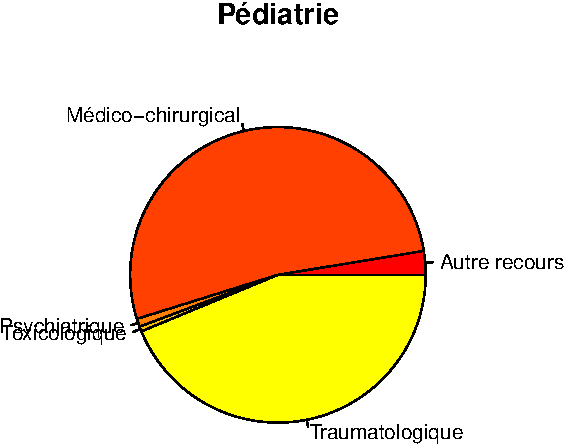
\includegraphics{analyse_merge_files/figure-latex/ped-1.pdf}

\begin{Shaded}
\begin{Highlighting}[]
\NormalTok{tabp <-}\StringTok{ }\KeywordTok{tab1}\NormalTok{(d3p$TYPE_URGENCES, }\DataTypeTok{sort.group =} \StringTok{"decreasing"}\NormalTok{, }\DataTypeTok{bar.values =} \StringTok{"percent"}\NormalTok{, }\DataTypeTok{cex.names =} \FloatTok{0.8}\NormalTok{, }\DataTypeTok{main =} \KeywordTok{paste0}\NormalTok{(}\StringTok{"Médico-chirurgical pédiatrique (N = "}\NormalTok{, n.ped, }\StringTok{")"}\NormalTok{), }\DataTypeTok{missing =} \OtherTok{FALSE}\NormalTok{)}
\end{Highlighting}
\end{Shaded}

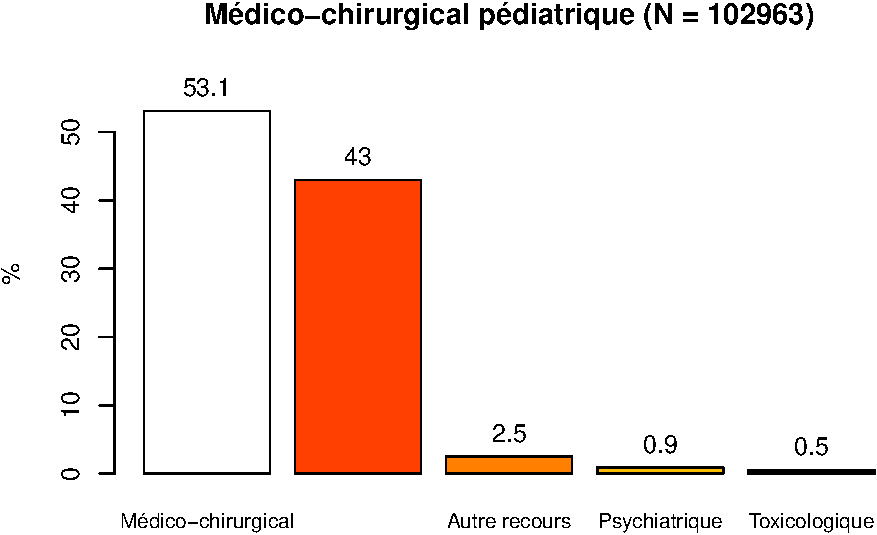
\includegraphics{analyse_merge_files/figure-latex/ped-2.pdf}

\subsection{Gériatrie (age \textgreater{} 75
ans)}\label{geriatrie-age-75-ans}

\begin{Shaded}
\begin{Highlighting}[]
\NormalTok{d3g <-}\StringTok{ }\NormalTok{d3[d3$AGE >}\StringTok{ }\DecValTok{75}\NormalTok{,]}
\NormalTok{n.ger <-}\StringTok{ }\KeywordTok{nrow}\NormalTok{(d3g)}

\NormalTok{s.type.ger <-}\StringTok{ }\KeywordTok{table}\NormalTok{(d3g$TYPE_URGENCES)}
\KeywordTok{sort}\NormalTok{(s.type.ger, }\DataTypeTok{decreasing =} \OtherTok{TRUE}\NormalTok{)}
\end{Highlighting}
\end{Shaded}

\begin{verbatim}
## 
## Médico-chirurgical    Traumatologique      Autre recours 
##              22198               8500                533 
##      Psychiatrique      Toxicologique 
##                376                163
\end{verbatim}

\begin{Shaded}
\begin{Highlighting}[]
\KeywordTok{pie}\NormalTok{(}\KeywordTok{sort}\NormalTok{(s.type.ger), }\DataTypeTok{main =} \StringTok{"Gériatrie"}\NormalTok{, }\DataTypeTok{cex=}\FloatTok{0.8}\NormalTok{, }\DataTypeTok{col =} \KeywordTok{palette}\NormalTok{(}\KeywordTok{heat.colors}\NormalTok{(}\DecValTok{6}\NormalTok{)))}
\end{Highlighting}
\end{Shaded}

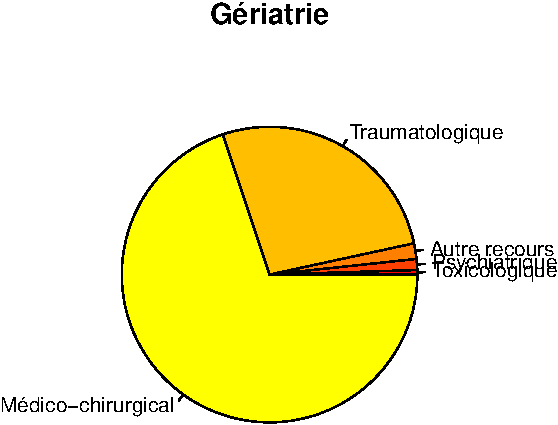
\includegraphics{analyse_merge_files/figure-latex/geriatrie-1.pdf}

\begin{Shaded}
\begin{Highlighting}[]
\NormalTok{tabp <-}\StringTok{ }\KeywordTok{tab1}\NormalTok{(d3g$TYPE_URGENCES, }\DataTypeTok{sort.group =} \StringTok{"decreasing"}\NormalTok{, }\DataTypeTok{bar.values =} \StringTok{"percent"}\NormalTok{, }\DataTypeTok{cex.names =} \FloatTok{0.8}\NormalTok{, }\DataTypeTok{main =} \KeywordTok{paste0}\NormalTok{(}\StringTok{"Médico-chirurgical gériatrique (N = "}\NormalTok{, n.ger, }\StringTok{")"}\NormalTok{), }\DataTypeTok{missing =} \OtherTok{FALSE}\NormalTok{)}
\end{Highlighting}
\end{Shaded}

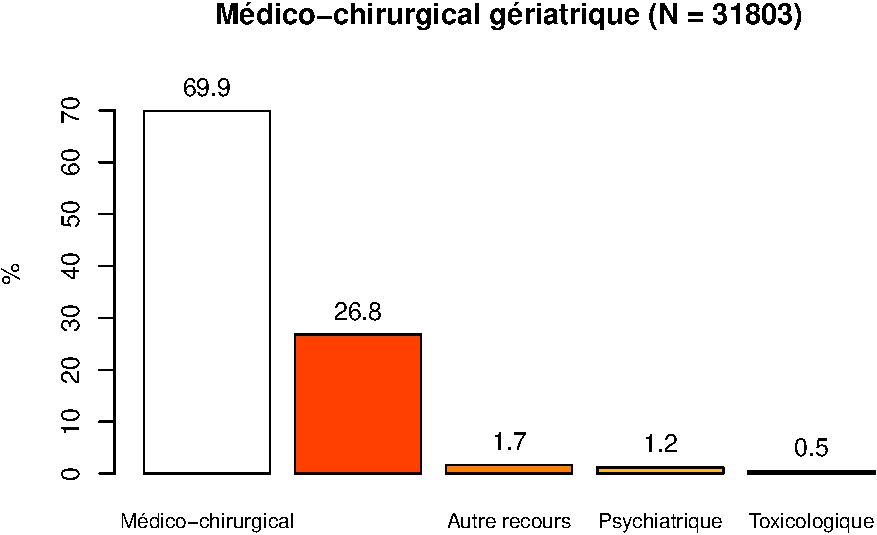
\includegraphics{analyse_merge_files/figure-latex/geriatrie-2.pdf}

\subsection{Synthèse}\label{synthese}

\begin{Shaded}
\begin{Highlighting}[]
\CommentTok{# table de regroupement}
\NormalTok{t.type <-}\StringTok{ }\KeywordTok{rbind}\NormalTok{(s.type.adl, s.type.ped, s.type.ger)}
\NormalTok{t.type}
\end{Highlighting}
\end{Shaded}

\begin{verbatim}
##            Autre recours Médico-chirurgical Psychiatrique Toxicologique
## s.type.adl          5375              80448          4532          3546
## s.type.ped          2237              45173           768           471
## s.type.ger           533              22198           376           163
##            Traumatologique
## s.type.adl           53216
## s.type.ped           37842
## s.type.ger            8500
\end{verbatim}

\begin{Shaded}
\begin{Highlighting}[]
\KeywordTok{barplot}\NormalTok{(t.type)}
\end{Highlighting}
\end{Shaded}

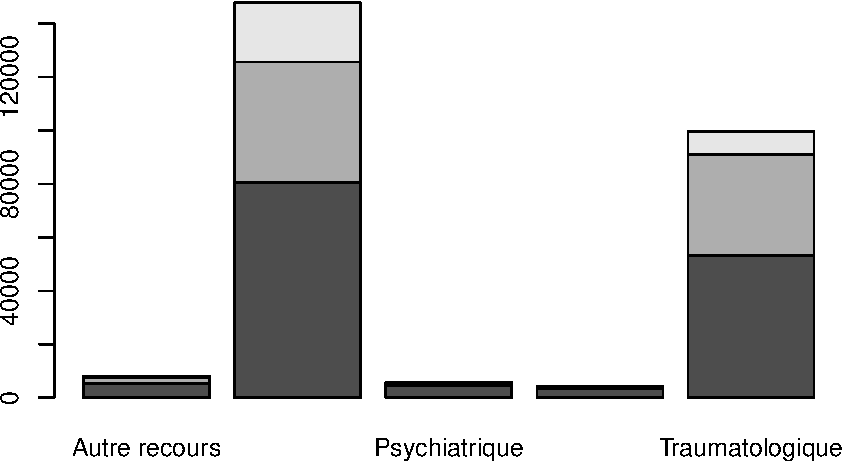
\includegraphics{analyse_merge_files/figure-latex/synthese-1.pdf}

\begin{Shaded}
\begin{Highlighting}[]
\CommentTok{# en pourcentages}
\NormalTok{p.type <-}\StringTok{ }\KeywordTok{round}\NormalTok{(}\KeywordTok{prop.table}\NormalTok{(t.type, }\DataTypeTok{margin =} \DecValTok{1}\NormalTok{)*}\DecValTok{100}\NormalTok{, }\DecValTok{2}\NormalTok{)}
\NormalTok{p.type}
\end{Highlighting}
\end{Shaded}

\begin{verbatim}
##            Autre recours Médico-chirurgical Psychiatrique Toxicologique
## s.type.adl          3.65              54.68          3.08          2.41
## s.type.ped          2.59              52.23          0.89          0.54
## s.type.ger          1.68              69.87          1.18          0.51
##            Traumatologique
## s.type.adl           36.17
## s.type.ped           43.75
## s.type.ger           26.75
\end{verbatim}

\begin{Shaded}
\begin{Highlighting}[]
\NormalTok{color <-}\StringTok{ }\KeywordTok{c}\NormalTok{(}\StringTok{"red"}\NormalTok{, }\StringTok{"green"}\NormalTok{, }\StringTok{"yellow"}\NormalTok{)}
\KeywordTok{barplot}\NormalTok{(p.type, }\DataTypeTok{cex.names =} \FloatTok{0.6}\NormalTok{)}
\end{Highlighting}
\end{Shaded}

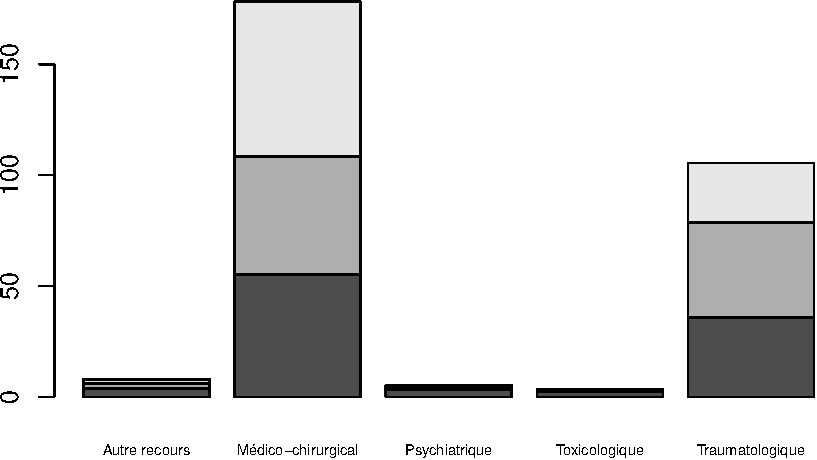
\includegraphics{analyse_merge_files/figure-latex/synthese-2.pdf}

\begin{Shaded}
\begin{Highlighting}[]
\KeywordTok{barplot}\NormalTok{(p.type, }\DataTypeTok{cex.names =} \FloatTok{0.6}\NormalTok{, }\DataTypeTok{beside =} \OtherTok{TRUE}\NormalTok{, }\DataTypeTok{col =} \NormalTok{color, }\DataTypeTok{main =} \StringTok{"Pathologies selon l'age"}\NormalTok{)}
\KeywordTok{legend}\NormalTok{(}\StringTok{"topright"}\NormalTok{, }\DataTypeTok{legend =} \KeywordTok{c}\NormalTok{(}\StringTok{"18-75 ans"}\NormalTok{,}\StringTok{"0-18 ans"}\NormalTok{,}\StringTok{"Sup.75 ans"}\NormalTok{), }\DataTypeTok{col =} \NormalTok{color, }\DataTypeTok{pch =} \DecValTok{15}\NormalTok{)}
\end{Highlighting}
\end{Shaded}

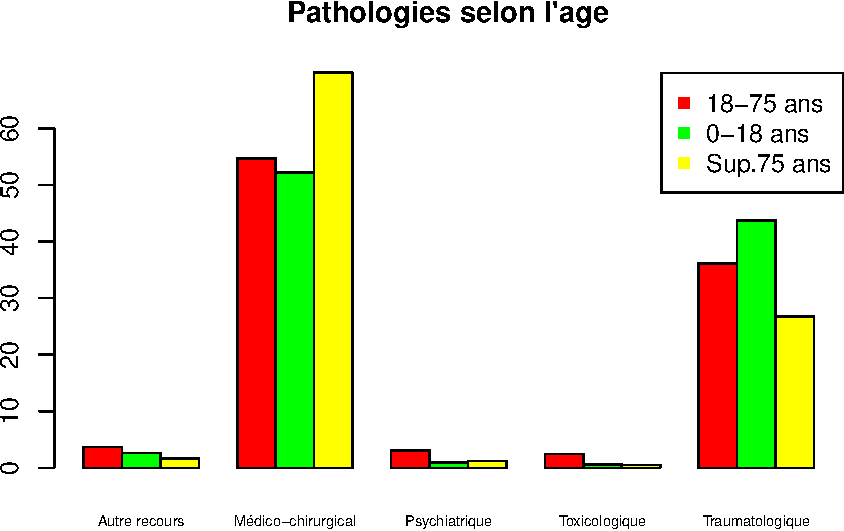
\includegraphics{analyse_merge_files/figure-latex/synthese-3.pdf}

\section{Par chapitre}\label{par-chapitre}

\subsection{Adultes}\label{adultes}

\subsubsection{Pathologie
médico-chirurgicale}\label{pathologie-medico-chirurgicale}

\begin{Shaded}
\begin{Highlighting}[]
\NormalTok{medic.adl <-}\StringTok{ }\NormalTok{d3a[d3a$TYPE_URGENCES ==}\StringTok{ "Médico-chirurgical"}\NormalTok{,]}
\NormalTok{n.medic.adl <-}\StringTok{ }\KeywordTok{nrow}\NormalTok{(medic.adl)}
\NormalTok{s.medic.adl <-}\StringTok{ }\KeywordTok{table}\NormalTok{(}\KeywordTok{factor}\NormalTok{(medic.adl$CHAPITRE))}
\NormalTok{p.medic.adl <-}\StringTok{ }\KeywordTok{round}\NormalTok{(}\KeywordTok{prop.table}\NormalTok{(s.medic.adl)*}\DecValTok{100}\NormalTok{, }\DecValTok{2}\NormalTok{)}
\KeywordTok{sort}\NormalTok{(p.medic.adl, }\DataTypeTok{decreasing =} \OtherTok{TRUE}\NormalTok{)}
\end{Highlighting}
\end{Shaded}

\begin{verbatim}
## 
##            Douleurs de membre, rhumatologie, orthopédie, SNP 
##                                                        18.61 
##                 Douleurs abdominales, pathologies digestives 
##                                                        17.36 
##            ORL, ophtalmo, stomato et carrefour aéro-digestif 
##                                                         9.66 
##               Douleurs pelviennes, pathologies uro-génitales 
##                                                         9.30 
##         Douleurs thoraciques, pathologies cardio-vasculaires 
##                                                         8.61 
##                Céphalées, pathologies neurologiques hors SNP 
##                                                         7.81 
##          Dermato-allergologie et atteintes cutanéo-muqueuses 
##                                                         7.12 
##                        Signes généraux et autres pathologies 
##                                                         6.58 
## Malaises, lipothymies, syncopes, étourdissements et vertiges 
##                                                         6.27 
##        Dyspnées, pathologies des voies aériennes inférieures 
##                                                         6.20 
##                             Fièvre et infectiologie générale 
##                                                         2.48
\end{verbatim}

\begin{Shaded}
\begin{Highlighting}[]
\KeywordTok{tab1}\NormalTok{(}\KeywordTok{factor}\NormalTok{(medic.adl$CHAPITRE), }\DataTypeTok{cex.names =} \FloatTok{0.5}\NormalTok{, }\DataTypeTok{cex =} \FloatTok{0.8}\NormalTok{, }\DataTypeTok{sort.group =} \StringTok{"decreasing"}\NormalTok{, }\DataTypeTok{main =} \StringTok{"Médico-chir adultes"}\NormalTok{, }\DataTypeTok{bar.values =} \StringTok{"percent"}\NormalTok{)}
\end{Highlighting}
\end{Shaded}

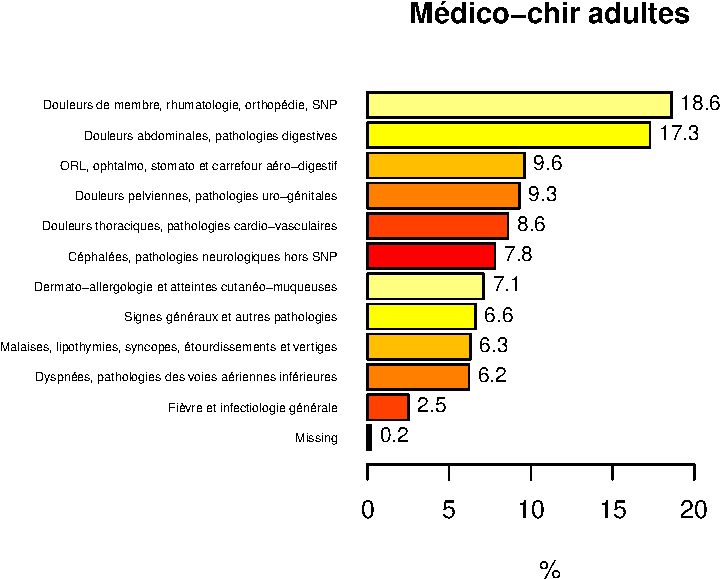
\includegraphics{analyse_merge_files/figure-latex/chap_adultes-1.pdf}

\begin{verbatim}
## factor(medic.adl$CHAPITRE) : 
##                                                              Frequency
## Douleurs de membre, rhumatologie, orthopédie, SNP                14972
## Douleurs abdominales, pathologies digestives                     13964
## ORL, ophtalmo, stomato et carrefour aéro-digestif                 7775
## Douleurs pelviennes, pathologies uro-génitales                    7480
## Douleurs thoraciques, pathologies cardio-vasculaires              6927
## Céphalées, pathologies neurologiques hors SNP                     6286
## Dermato-allergologie et atteintes cutanéo-muqueuses               5727
## Signes généraux et autres pathologies                             5293
## Malaises, lipothymies, syncopes, étourdissements et vertiges      5043
## Dyspnées, pathologies des voies aériennes inférieures             4984
## Fièvre et infectiologie générale                                  1997
## NA's                                                               182
##   Total                                                          80630
##                                                                %(NA+)
## Douleurs de membre, rhumatologie, orthopédie, SNP                18.6
## Douleurs abdominales, pathologies digestives                     17.3
## ORL, ophtalmo, stomato et carrefour aéro-digestif                 9.6
## Douleurs pelviennes, pathologies uro-génitales                    9.3
## Douleurs thoraciques, pathologies cardio-vasculaires              8.6
## Céphalées, pathologies neurologiques hors SNP                     7.8
## Dermato-allergologie et atteintes cutanéo-muqueuses               7.1
## Signes généraux et autres pathologies                             6.6
## Malaises, lipothymies, syncopes, étourdissements et vertiges      6.3
## Dyspnées, pathologies des voies aériennes inférieures             6.2
## Fièvre et infectiologie générale                                  2.5
## NA's                                                              0.2
##   Total                                                         100.0
##                                                                %(NA-)
## Douleurs de membre, rhumatologie, orthopédie, SNP                18.6
## Douleurs abdominales, pathologies digestives                     17.4
## ORL, ophtalmo, stomato et carrefour aéro-digestif                 9.7
## Douleurs pelviennes, pathologies uro-génitales                    9.3
## Douleurs thoraciques, pathologies cardio-vasculaires              8.6
## Céphalées, pathologies neurologiques hors SNP                     7.8
## Dermato-allergologie et atteintes cutanéo-muqueuses               7.1
## Signes généraux et autres pathologies                             6.6
## Malaises, lipothymies, syncopes, étourdissements et vertiges      6.3
## Dyspnées, pathologies des voies aériennes inférieures             6.2
## Fièvre et infectiologie générale                                  2.5
## NA's                                                              0.0
##   Total                                                         100.0
\end{verbatim}

\subsubsection{Pathologie traumatique}\label{pathologie-traumatique}

\begin{Shaded}
\begin{Highlighting}[]
\NormalTok{trauma.adl <-}\StringTok{ }\NormalTok{d3a[d3a$TYPE_URGENCES ==}\StringTok{ "Traumatologique"}\NormalTok{,]}
\NormalTok{n.trauma.adl <-}\StringTok{ }\KeywordTok{nrow}\NormalTok{(trauma.adl)}
\NormalTok{s.trauma.adl <-}\StringTok{ }\KeywordTok{table}\NormalTok{(}\KeywordTok{factor}\NormalTok{(trauma.adl$CHAPITRE))}
\NormalTok{p.trauma.adl <-}\StringTok{ }\KeywordTok{round}\NormalTok{(}\KeywordTok{prop.table}\NormalTok{(s.trauma.adl)*}\DecValTok{100}\NormalTok{, }\DecValTok{2}\NormalTok{)}
\KeywordTok{sort}\NormalTok{(p.trauma.adl, }\DataTypeTok{decreasing =} \OtherTok{TRUE}\NormalTok{)}
\end{Highlighting}
\end{Shaded}

\begin{verbatim}
## 
##      Traumatisme du membre supérieur      Traumatisme du membre inférieur 
##                                37.75                                31.30 
##     Traumatisme de la tête et du cou Traumatisme thoraco-abdomino-pelvien 
##                                16.75                                 7.11 
##  Traumatisme autre et sans précision 
##                                 7.10
\end{verbatim}

\begin{Shaded}
\begin{Highlighting}[]
\KeywordTok{tab1}\NormalTok{(}\KeywordTok{factor}\NormalTok{(trauma.adl$CHAPITRE), }\DataTypeTok{cex.names =} \FloatTok{0.5}\NormalTok{, }\DataTypeTok{cex =} \FloatTok{0.8}\NormalTok{, }\DataTypeTok{sort.group =} \StringTok{"decreasing"}\NormalTok{, }\DataTypeTok{main =} \StringTok{"Traumatologie adultes"}\NormalTok{, }\DataTypeTok{bar.values =} \StringTok{"percent"}\NormalTok{, }\DataTypeTok{horiz =} \OtherTok{TRUE}\NormalTok{)}
\end{Highlighting}
\end{Shaded}

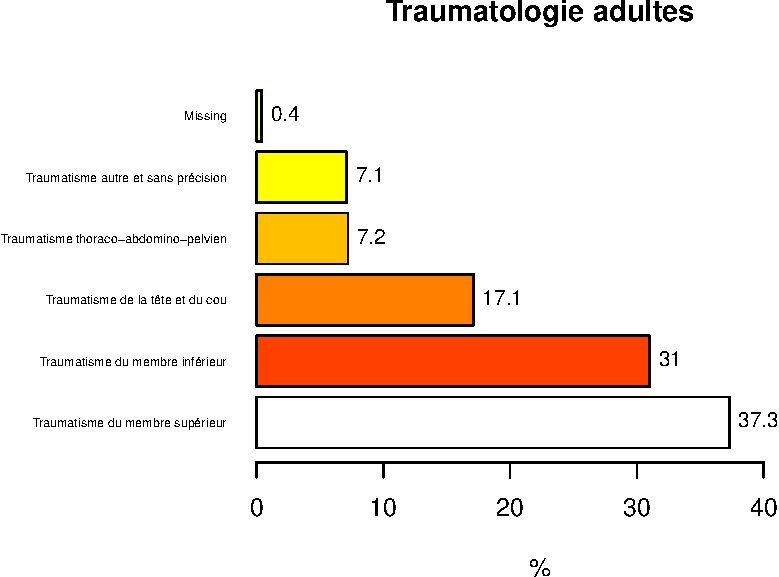
\includegraphics{analyse_merge_files/figure-latex/trauma_adulte-1.pdf}

\begin{verbatim}
## factor(trauma.adl$CHAPITRE) : 
##                                      Frequency   %(NA+)   %(NA-)
## Traumatisme du membre supérieur          20089     37.6     37.7
## Traumatisme du membre inférieur          16656     31.2     31.3
## Traumatisme de la tête et du cou          8912     16.7     16.7
## Traumatisme thoraco-abdomino-pelvien      3781      7.1      7.1
## Traumatisme autre et sans précision       3778      7.1      7.1
## NA's                                       182      0.3      0.0
##   Total                                  53398    100.0    100.0
\end{verbatim}

\subsection{Enfants}\label{enfants}

\subsubsection{Pathologie médico-chirurgicale
pédiatrique}\label{pathologie-medico-chirurgicale-pediatrique}

\begin{Shaded}
\begin{Highlighting}[]
\NormalTok{f <-}\StringTok{ }\KeywordTok{groupe.pathologique}\NormalTok{(d3p, }\StringTok{"medchir"}\NormalTok{)}
\KeywordTok{tab1}\NormalTok{(f$data, }\DataTypeTok{cex.names =} \FloatTok{0.5}\NormalTok{, }\DataTypeTok{cex =} \FloatTok{0.8}\NormalTok{, }\DataTypeTok{sort.group =} \StringTok{"decreasing"}\NormalTok{, }\DataTypeTok{main =} \StringTok{"Médico-chir pédiatrique"}\NormalTok{, }\DataTypeTok{bar.values =} \StringTok{"percent"}\NormalTok{)}
\end{Highlighting}
\end{Shaded}

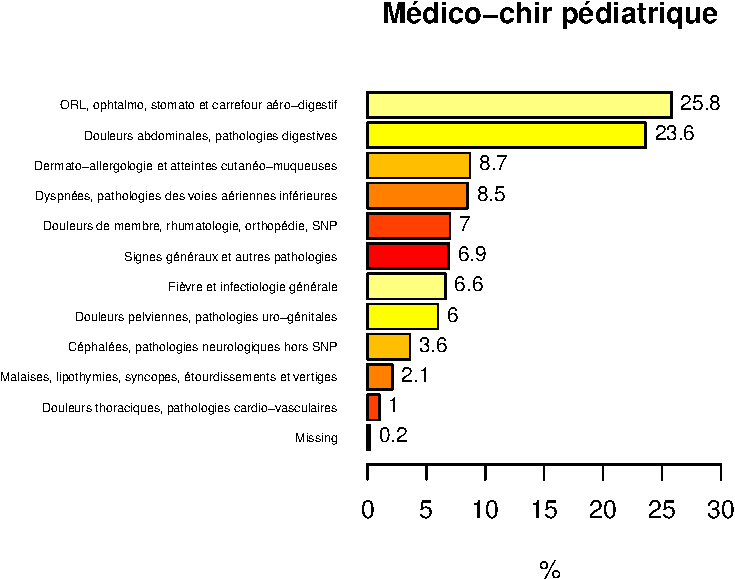
\includegraphics{analyse_merge_files/figure-latex/chap_ped_med-1.pdf}

\begin{verbatim}
## f$data : 
##                                                              Frequency
## ORL, ophtalmo, stomato et carrefour aéro-digestif                11343
## Douleurs abdominales, pathologies digestives                     10908
## Dermato-allergologie et atteintes cutanéo-muqueuses               4063
## Dyspnées, pathologies des voies aériennes inférieures             3422
## Fièvre et infectiologie générale                                  3185
## Douleurs de membre, rhumatologie, orthopédie, SNP                 3172
## Signes généraux et autres pathologies                             3172
## Douleurs pelviennes, pathologies uro-génitales                    2816
## Céphalées, pathologies neurologiques hors SNP                     1670
## Malaises, lipothymies, syncopes, étourdissements et vertiges       962
## Douleurs thoraciques, pathologies cardio-vasculaires               460
## NA's                                                                84
##   Total                                                          45257
##                                                                %(NA+)
## ORL, ophtalmo, stomato et carrefour aéro-digestif                25.1
## Douleurs abdominales, pathologies digestives                     24.1
## Dermato-allergologie et atteintes cutanéo-muqueuses               9.0
## Dyspnées, pathologies des voies aériennes inférieures             7.6
## Fièvre et infectiologie générale                                  7.0
## Douleurs de membre, rhumatologie, orthopédie, SNP                 7.0
## Signes généraux et autres pathologies                             7.0
## Douleurs pelviennes, pathologies uro-génitales                    6.2
## Céphalées, pathologies neurologiques hors SNP                     3.7
## Malaises, lipothymies, syncopes, étourdissements et vertiges      2.1
## Douleurs thoraciques, pathologies cardio-vasculaires              1.0
## NA's                                                              0.2
##   Total                                                         100.0
##                                                                %(NA-)
## ORL, ophtalmo, stomato et carrefour aéro-digestif                25.1
## Douleurs abdominales, pathologies digestives                     24.1
## Dermato-allergologie et atteintes cutanéo-muqueuses               9.0
## Dyspnées, pathologies des voies aériennes inférieures             7.6
## Fièvre et infectiologie générale                                  7.1
## Douleurs de membre, rhumatologie, orthopédie, SNP                 7.0
## Signes généraux et autres pathologies                             7.0
## Douleurs pelviennes, pathologies uro-génitales                    6.2
## Céphalées, pathologies neurologiques hors SNP                     3.7
## Malaises, lipothymies, syncopes, étourdissements et vertiges      2.1
## Douleurs thoraciques, pathologies cardio-vasculaires              1.0
## NA's                                                              0.0
##   Total                                                         100.0
\end{verbatim}

\subsubsection{Pathologie traumatique
pédiatrique}\label{pathologie-traumatique-pediatrique}

\begin{Shaded}
\begin{Highlighting}[]
\NormalTok{f <-}\StringTok{ }\KeywordTok{groupe.pathologique}\NormalTok{(d3p, }\StringTok{"trau"}\NormalTok{)}
\KeywordTok{tab1}\NormalTok{(f$data, }\DataTypeTok{cex.names =} \FloatTok{0.5}\NormalTok{, }\DataTypeTok{cex =} \FloatTok{0.8}\NormalTok{, }\DataTypeTok{sort.group =} \StringTok{"decreasing"}\NormalTok{, }\DataTypeTok{main =} \StringTok{"Traumatologie pédiatrique"}\NormalTok{, }\DataTypeTok{bar.values =} \StringTok{"percent"}\NormalTok{)}
\end{Highlighting}
\end{Shaded}

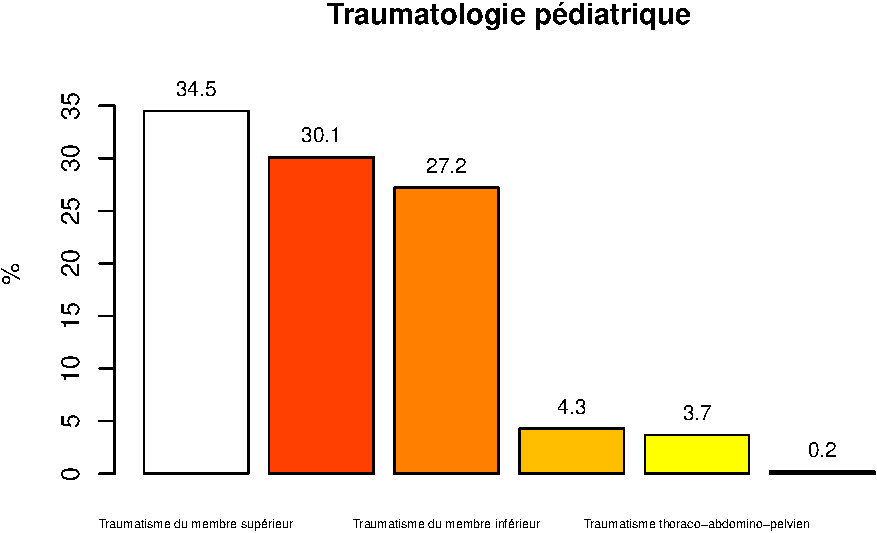
\includegraphics{analyse_merge_files/figure-latex/chap_ped_trau-1.pdf}

\begin{verbatim}
## f$data : 
##                                      Frequency   %(NA+)   %(NA-)
## Traumatisme du membre supérieur          13072     34.5     34.5
## Traumatisme de la tête et du cou         11398     30.1     30.1
## Traumatisme du membre inférieur          10316     27.2     27.3
## Traumatisme autre et sans précision       1644      4.3      4.3
## Traumatisme thoraco-abdomino-pelvien      1412      3.7      3.7
## NA's                                        84      0.2      0.0
##   Total                                  37926    100.0    100.0
\end{verbatim}

\subsection{Gériatrie}\label{geriatrie}

\subsubsection{Pathologie médico-chirurgicale
gériatrique}\label{pathologie-medico-chirurgicale-geriatrique}

\begin{Shaded}
\begin{Highlighting}[]
\NormalTok{f <-}\StringTok{ }\KeywordTok{groupe.pathologique}\NormalTok{(d3g, }\StringTok{"medchir"}\NormalTok{)}
\KeywordTok{tab1}\NormalTok{(f$data, }\DataTypeTok{cex.names =} \FloatTok{0.5}\NormalTok{, }\DataTypeTok{cex =} \FloatTok{0.8}\NormalTok{, }\DataTypeTok{sort.group =} \StringTok{"decreasing"}\NormalTok{, }\DataTypeTok{main =} \StringTok{"Médico-chir gériatrique"}\NormalTok{, }\DataTypeTok{bar.values =} \StringTok{"percent"}\NormalTok{)}
\end{Highlighting}
\end{Shaded}

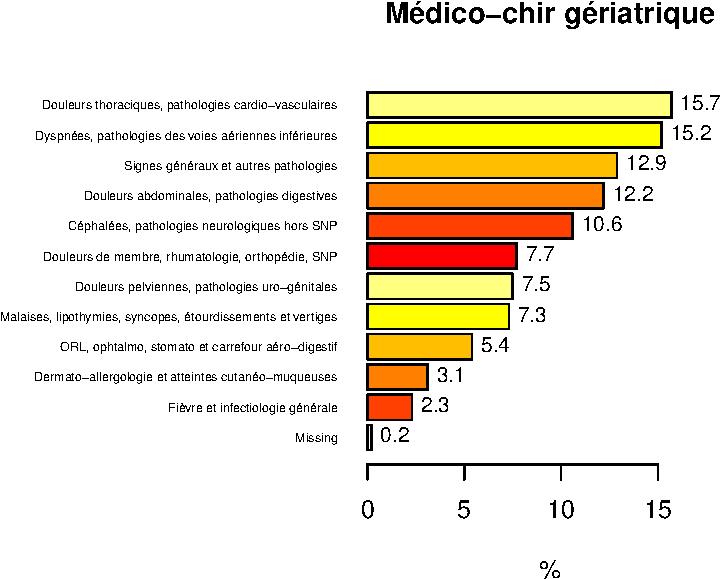
\includegraphics{analyse_merge_files/figure-latex/chap_ger_med-1.pdf}

\begin{verbatim}
## f$data : 
##                                                              Frequency
## Douleurs thoraciques, pathologies cardio-vasculaires              3471
## Dyspnées, pathologies des voies aériennes inférieures             3414
## Signes généraux et autres pathologies                             2898
## Douleurs abdominales, pathologies digestives                      2708
## Céphalées, pathologies neurologiques hors SNP                     2346
## Douleurs de membre, rhumatologie, orthopédie, SNP                 1690
## Douleurs pelviennes, pathologies uro-génitales                    1634
## Malaises, lipothymies, syncopes, étourdissements et vertiges      1627
## ORL, ophtalmo, stomato et carrefour aéro-digestif                 1216
## Dermato-allergologie et atteintes cutanéo-muqueuses                674
## Fièvre et infectiologie générale                                   520
## NA's                                                                33
##   Total                                                          22231
##                                                                %(NA+)
## Douleurs thoraciques, pathologies cardio-vasculaires             15.6
## Dyspnées, pathologies des voies aériennes inférieures            15.4
## Signes généraux et autres pathologies                            13.0
## Douleurs abdominales, pathologies digestives                     12.2
## Céphalées, pathologies neurologiques hors SNP                    10.6
## Douleurs de membre, rhumatologie, orthopédie, SNP                 7.6
## Douleurs pelviennes, pathologies uro-génitales                    7.4
## Malaises, lipothymies, syncopes, étourdissements et vertiges      7.3
## ORL, ophtalmo, stomato et carrefour aéro-digestif                 5.5
## Dermato-allergologie et atteintes cutanéo-muqueuses               3.0
## Fièvre et infectiologie générale                                  2.3
## NA's                                                              0.1
##   Total                                                         100.0
##                                                                %(NA-)
## Douleurs thoraciques, pathologies cardio-vasculaires             15.6
## Dyspnées, pathologies des voies aériennes inférieures            15.4
## Signes généraux et autres pathologies                            13.1
## Douleurs abdominales, pathologies digestives                     12.2
## Céphalées, pathologies neurologiques hors SNP                    10.6
## Douleurs de membre, rhumatologie, orthopédie, SNP                 7.6
## Douleurs pelviennes, pathologies uro-génitales                    7.4
## Malaises, lipothymies, syncopes, étourdissements et vertiges      7.3
## ORL, ophtalmo, stomato et carrefour aéro-digestif                 5.5
## Dermato-allergologie et atteintes cutanéo-muqueuses               3.0
## Fièvre et infectiologie générale                                  2.3
## NA's                                                              0.0
##   Total                                                         100.0
\end{verbatim}

\subsubsection{Pathologie traumatique
gériatrique}\label{pathologie-traumatique-geriatrique}

\begin{Shaded}
\begin{Highlighting}[]
\NormalTok{f <-}\StringTok{ }\KeywordTok{groupe.pathologique}\NormalTok{(d3g, }\StringTok{"trau"}\NormalTok{)}
\KeywordTok{tab1}\NormalTok{(f$data, }\DataTypeTok{cex.names =} \FloatTok{0.5}\NormalTok{, }\DataTypeTok{cex =} \FloatTok{0.8}\NormalTok{, }\DataTypeTok{sort.group =} \StringTok{"decreasing"}\NormalTok{, }\DataTypeTok{main =} \StringTok{"Traumatologie gériatrique"}\NormalTok{, }\DataTypeTok{bar.values =} \StringTok{"percent"}\NormalTok{)}
\end{Highlighting}
\end{Shaded}

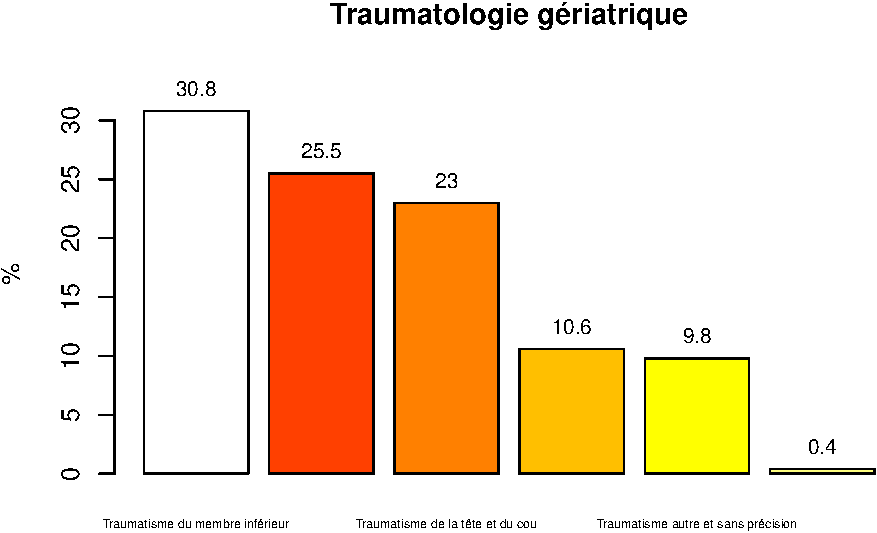
\includegraphics{analyse_merge_files/figure-latex/chap_ger_trau-1.pdf}

\begin{verbatim}
## f$data : 
##                                      Frequency   %(NA+)   %(NA-)
## Traumatisme du membre inférieur           2627     30.8     30.9
## Traumatisme du membre supérieur           2179     25.5     25.6
## Traumatisme de la tête et du cou          1961     23.0     23.1
## Traumatisme thoraco-abdomino-pelvien       901     10.6     10.6
## Traumatisme autre et sans précision        832      9.8      9.8
## NA's                                        33      0.4      0.0
##   Total                                   8533    100.0    100.0
\end{verbatim}

\subsection{Synthèse}\label{synthese-1}

Passages bruts:

\begin{verbatim}
Warning in rbind(s.type.ped, s.type.adl, s.type.ger, s.type): number of
columns of result is not a multiple of vector length (arg 1)
\end{verbatim}

\begin{verbatim}
               Autre recours Médico-chirurgical Psychiatrique
< 18 ans                2237              45173           768
18-74 ans               5375              80448          4532
75 ans et plus           533              22198           376
TOTAL                   8145             147819          5677
               Toxicologique Traumatologique NA's
< 18 ans                 471           37842 2237
18-74 ans               3546           53216 5375
75 ans et plus           163            8500  533
TOTAL                   4180           99558  296
\end{verbatim}

Taux de passage standardisé pour 1000 RPU:

\begin{verbatim}
Warning in rbind(t1, t2, t3, t4): number of columns of result is not a
multiple of vector length (arg 1)
\end{verbatim}

\begin{verbatim}
               Autre recours Médico-chirurgical Psychiatrique
< 18 ans               25.86             522.29          8.88
18-74 ans              36.54             546.83         30.81
75 ans et plus         16.78             698.71         11.84
TOTAL                  30.66             556.39         21.37
               Toxicologique Traumatologique  NA's
< 18 ans                5.45          437.53 25.86
18-74 ans              24.10          361.73 36.54
75 ans et plus          5.13          267.55 16.78
TOTAL                  15.73          374.74  1.11
\end{verbatim}

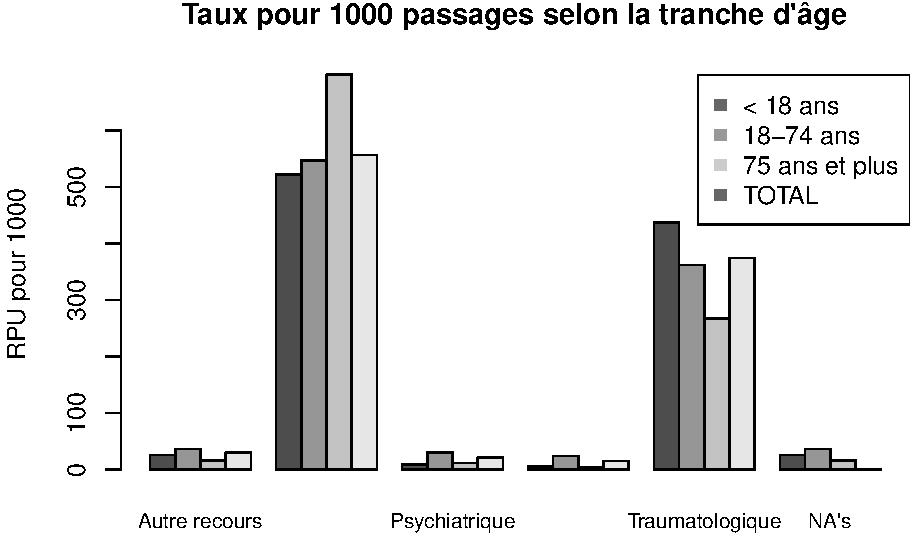
\includegraphics{analyse_merge_files/figure-latex/synthese2-1.pdf}

\section{AVC}\label{avc}

\begin{Shaded}
\begin{Highlighting}[]
\NormalTok{AVC<-d3[}\KeywordTok{substr}\NormalTok{(d3$DP,}\DecValTok{1}\NormalTok{,}\DecValTok{3}\NormalTok{)>=}\StringTok{"I60"} \NormalTok{&}\StringTok{ }\KeywordTok{substr}\NormalTok{(d3$DP,}\DecValTok{1}\NormalTok{,}\DecValTok{3}\NormalTok{)<}\StringTok{"I65"} \NormalTok{|}\StringTok{ }\KeywordTok{substr}\NormalTok{(d3$DP,}\DecValTok{1}\NormalTok{,}\DecValTok{3}\NormalTok{)==}\StringTok{"G46"} \NormalTok{|}\StringTok{ }\KeywordTok{substr}\NormalTok{(d3$DP,}\DecValTok{1}\NormalTok{,}\DecValTok{3}\NormalTok{)==}\StringTok{"G45"} \NormalTok{,]}
\NormalTok{AVC$etiologie <-}\StringTok{ }\OtherTok{NA}
\NormalTok{AVC$etiologie[}\KeywordTok{substr}\NormalTok{(AVC$DP,}\DecValTok{1}\NormalTok{,}\DecValTok{3}\NormalTok{) %in%}\StringTok{ }\KeywordTok{c}\NormalTok{(}\StringTok{"I60"}\NormalTok{,}\StringTok{"I61"}\NormalTok{,}\StringTok{"I62"}\NormalTok{)] <-}\StringTok{"HEMO"}
\NormalTok{AVC$etiologie[}\KeywordTok{substr}\NormalTok{(AVC$DP,}\DecValTok{1}\NormalTok{,}\DecValTok{3}\NormalTok{) %in%}\StringTok{ }\KeywordTok{c}\NormalTok{(}\StringTok{"I63"}\NormalTok{,}\StringTok{"I64"}\NormalTok{)] <-}\StringTok{"ISCH"}
\NormalTok{AVC$etiologie[}\KeywordTok{substr}\NormalTok{(AVC$DP,}\DecValTok{1}\NormalTok{,}\DecValTok{3}\NormalTok{) %in%}\StringTok{ }\KeywordTok{c}\NormalTok{(}\StringTok{"I64"}\NormalTok{)] <-}\StringTok{"NPRE"}
\NormalTok{AVC$etiologie[}\KeywordTok{substr}\NormalTok{(AVC$DP,}\DecValTok{1}\NormalTok{,}\DecValTok{3}\NormalTok{) %in%}\StringTok{ }\KeywordTok{c}\NormalTok{(}\StringTok{"G45"}\NormalTok{,}\StringTok{"G46"}\NormalTok{)] <-}\StringTok{"AIT"}
\NormalTok{AVC$etiologie <-}\StringTok{ }\KeywordTok{as.factor}\NormalTok{(AVC$etiologie)}

\NormalTok{n.avc <-}\StringTok{ }\KeywordTok{nrow}\NormalTok{(AVC)}
\end{Highlighting}
\end{Shaded}

\subsection{RECUEIL DES DONNÉES}\label{recueil-des-donnees}

\begin{itemize}
\itemsep1pt\parskip0pt\parsep0pt
\item
  Nombre d'AVC dans l'année (+ rappeler le pourcentage d'exhaustivité du
  DP par rapport au nombre de RPU): \textbf{2476}
\item
  Moyenne quotidienne d'AVC: \textbf{6.7835616 AVC/j}
\item
  \% d'AVC dans l'activité globale: \textbf{0.9319657 \%}
\end{itemize}

\subsection{PATIENTS}\label{patients}

\begin{verbatim}
## c.age
##     [0,5)    [5,10)   [10,15)   [15,20)   [20,25)   [25,30)   [30,35) 
##         4         5         1         7        20        20        26 
##   [35,40)   [40,45)   [45,50)   [50,55)   [55,60)   [60,65)   [65,70) 
##        35        50        88       119       148       195       246 
##   [70,75)   [75,80)   [80,85)   [85,90)   [90,95)  [95,100) [100,105) 
##       222       350       406       338       165        26         5 
## [105,110) [110,115) [115,120) 
##         0         0         0
\end{verbatim}

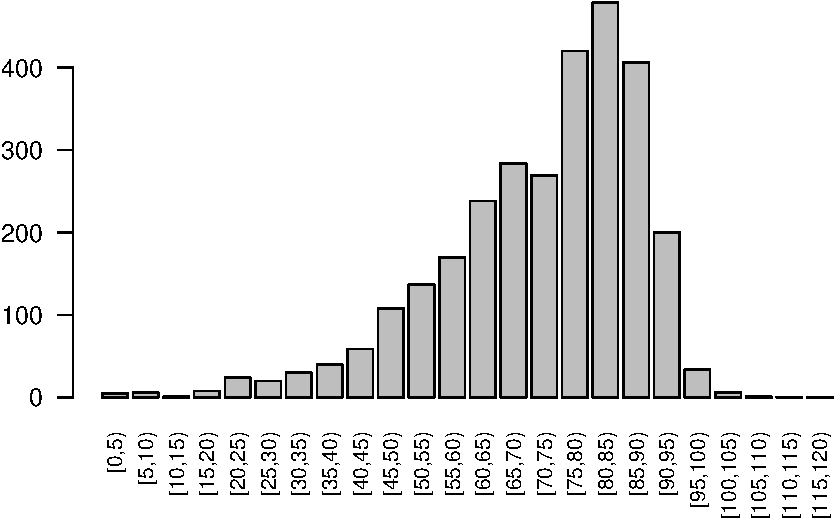
\includegraphics{analyse_merge_files/figure-latex/patients-1.pdf}

\begin{itemize}
\itemsep1pt\parskip0pt\parsep0pt
\item
  Sex ratio: 1.027846
\item
  Age moyen: 71.34 ans
\item
  Nombre d'AVC par sous classe d'âge (GT1):
\end{itemize}

\subsection{ARRIVÉE}\label{arrivee}

\begin{itemize}
\itemsep1pt\parskip0pt\parsep0pt
\item
  Nombre d'AVC et \% par tranche d'heure GT1 (matinée, début d'après
  midi, fin d'après midi, soirée, nuit profonde)
\end{itemize}

\begin{Shaded}
\begin{Highlighting}[]
\CommentTok{# heures de découpage}
\NormalTok{p <-}\StringTok{ }\KeywordTok{c}\NormalTok{(}\DecValTok{0}\NormalTok{, }\DecValTok{8}\NormalTok{, }\DecValTok{12}\NormalTok{, }\DecValTok{16}\NormalTok{, }\DecValTok{20}\NormalTok{, }\DecValTok{24}\NormalTok{)}
\CommentTok{# légende}
\NormalTok{np <-}\StringTok{ }\KeywordTok{c}\NormalTok{(}\StringTok{"nuit profonde"}\NormalTok{, }\StringTok{"matinée"}\NormalTok{, }\StringTok{"début après-midi"}\NormalTok{, }\StringTok{"fin après-midi"}\NormalTok{, }\StringTok{"soirée"}\NormalTok{)}
\CommentTok{# extraction des heures à partir du format datetime (http://stackoverflow.com/questions/19292438/split-date-time)}
\NormalTok{a <-}\StringTok{ }\KeywordTok{as.numeric}\NormalTok{(}\KeywordTok{format}\NormalTok{(}\KeywordTok{as.POSIXct}\NormalTok{(AVC$ENTREE), }\StringTok{"%H"}\NormalTok{))}

\NormalTok{x <-}\StringTok{ }\KeywordTok{cut}\NormalTok{(a, p, np, }\DataTypeTok{right =} \OtherTok{FALSE}\NormalTok{)}
\NormalTok{x2 <-}\StringTok{ }\KeywordTok{cut}\NormalTok{(a, p, }\DataTypeTok{right =} \OtherTok{FALSE}\NormalTok{)}

\KeywordTok{rbind}\NormalTok{(}\KeywordTok{levels}\NormalTok{(x2), }\KeywordTok{table}\NormalTok{(x))}
\end{Highlighting}
\end{Shaded}

\begin{verbatim}
##      nuit profonde matinée  début après-midi fin après-midi soirée   
## [1,] "[0,8)"       "[8,12)" "[12,16)"        "[16,20)"      "[20,24)"
## [2,] "226"         "783"    "778"            "495"          "194"
\end{verbatim}

\begin{Shaded}
\begin{Highlighting}[]
\KeywordTok{tab1}\NormalTok{(x, }\DataTypeTok{cex.names =} \FloatTok{0.8}\NormalTok{, }\DataTypeTok{main =} \StringTok{"Heure d'admission des AVC"}\NormalTok{, }\DataTypeTok{bar.values =} \StringTok{"percent"}\NormalTok{, }\DataTypeTok{ylab =} \StringTok{"%"}\NormalTok{)}
\end{Highlighting}
\end{Shaded}

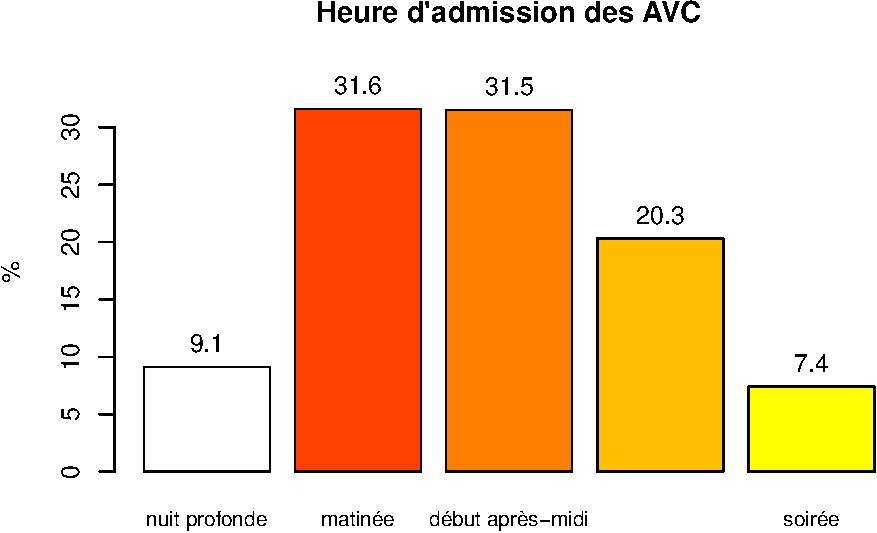
\includegraphics{analyse_merge_files/figure-latex/avc_periode-1.pdf}

\begin{verbatim}
## x : 
##                  Frequency Percent Cum. percent
## nuit profonde          226     9.1          9.1
## matinée                783    31.6         40.8
## début après-midi       778    31.4         72.2
## fin après-midi         495    20.0         92.2
## soirée                 194     7.8        100.0
##   Total               2476   100.0        100.0
\end{verbatim}

\begin{itemize}
\itemsep1pt\parskip0pt\parsep0pt
\item
  \% passages en horaire de PDS
\end{itemize}

PDSS = horaires de PDS en semaine, PDSWE = horaires de PDS le WE, NPDS =
hors horaire de PDS.

\subsection{Mode d'arrivée aux
urgences}\label{mode-darrivee-aux-urgences}

\begin{Shaded}
\begin{Highlighting}[]
\NormalTok{n.avc.moyen <-}\StringTok{ }\KeywordTok{summary}\NormalTok{(}\KeywordTok{factor}\NormalTok{(AVC$TRANSPORT))}
\NormalTok{n.avc.moyen}
\end{Highlighting}
\end{Shaded}

\begin{verbatim}
##  AMBU    FO  HELI PERSO  SMUR  VSAB  NA's 
##  1152     1    14   543    59   418   289
\end{verbatim}

\begin{Shaded}
\begin{Highlighting}[]
\NormalTok{p.avc.moyen <-}\StringTok{ }\KeywordTok{round}\NormalTok{(}\KeywordTok{prop.table}\NormalTok{(n.avc.moyen)*}\DecValTok{100}\NormalTok{, }\DecValTok{2}\NormalTok{)}
\NormalTok{p.avc.moyen}
\end{Highlighting}
\end{Shaded}

\begin{verbatim}
##  AMBU    FO  HELI PERSO  SMUR  VSAB  NA's 
## 46.53  0.04  0.57 21.93  2.38 16.88 11.67
\end{verbatim}

\begin{itemize}
\itemsep1pt\parskip0pt\parsep0pt
\item
  \% d'arrivées Moyen perso
\item
  \% d'arrivées SMUR
\item
  \% d'arrivées VSAV
\item
  \% d'arrivées ambulance privée NB : commentaire possible pour
  expliquer que la somme des 4 pourcentages ci dessus ne fait pas 100 \%
\end{itemize}

\subsection{DIAGNOSTIC PRINCIPAL}\label{diagnostic-principal}

\texttt{r   t.diag \textless{}- table(AVC\$etiologie)   p.diag \textless{}- prop.table(t.diag)*100}

\begin{itemize}
\itemsep1pt\parskip0pt\parsep0pt
\item
  Nombre d'AVC et \%
\item
  Nombre d'AIT et \%
\item
  Nombre de codes ``symptomatiques'' (hémiplégie, aphasie, amaurose,
  etc\ldots{}) et \%
\item
  Nombre d'autres hémorragies non traumatiques et \%
\end{itemize}

NB : se référer à l'annexe 4 pour les regroupements.

\subsection{DURÉE}\label{duree}

\begin{itemize}
\itemsep1pt\parskip0pt\parsep0pt
\item
  Durée de passage (HORS UHCD) : moyenne et médiane
\item
  \% de passages de moins de 4h
\end{itemize}

\subsection{MODE DE SORTIE}\label{mode-de-sortie}

\begin{itemize}
\itemsep1pt\parskip0pt\parsep0pt
\item
  \% d'hospitalisation
\item
  \% de mutation
\item
  \% de transfert
\item
  \% de retour à domicile
\end{itemize}

\section{Résultats par type
d'établissement}\label{resultats-par-type-detablissement}

La trame commune recueuille les éléments suivants:

\begin{verbatim}
                 Autre recours Médico-chirurgical Psychiatrique
SU SAMU CHU              25.86             522.29          8.88
SU SAMU non CHU        1056.00           18671.00       1416.00
SU SMUR non SAMU       4324.00           62965.00       2410.00
SU non SMUR            1793.00           26254.00        487.00
TOTAL                  8145.00          147819.00       5677.00
                 Toxicologique Traumatologique
SU SAMU CHU               5.45          437.53
SU SAMU non CHU         696.00         7819.00
SU SMUR non SAMU       1908.00        47641.00
SU non SMUR             200.00        25141.00
TOTAL                  4180.00        99558.00
\end{verbatim}

Une table des types

\begin{Shaded}
\begin{Highlighting}[]
\NormalTok{x <-}\StringTok{ }\KeywordTok{tapply}\NormalTok{(d3$TYPE_URGENCES, d3$FINESS, table ) }\CommentTok{# x est un vecteur de list}
\NormalTok{y <-}\StringTok{ }\NormalTok{x[-}\DecValTok{3}\NormalTok{] }\CommentTok{# on retire ste anne qui n'a aucun DP}
\NormalTok{z <-}\StringTok{ }\KeywordTok{matrix}\NormalTok{(}\KeywordTok{unlist}\NormalTok{(y), }\DataTypeTok{nrow =} \KeywordTok{length}\NormalTok{(y), }\DataTypeTok{ncol =} \DecValTok{5}\NormalTok{) }\CommentTok{# on transforme y en matrice. Pour en faire un data frame: df <- df <- data.frame(matrix(unlist(y), nrow=14, byrow=T),stringsAsFactors=FALSE). Source: http://stackoverflow.com/questions/4227223/r-list-to-data-frame}
\end{Highlighting}
\end{Shaded}

\begin{verbatim}
## Warning in matrix(unlist(y), nrow = length(y), ncol = 5): la longueur des
## données [85] n'est pas un diviseur ni un multiple du nombre de lignes [19]
\end{verbatim}

\begin{Shaded}
\begin{Highlighting}[]
\KeywordTok{rownames}\NormalTok{(z) <-}\StringTok{ }\KeywordTok{names}\NormalTok{(x[-}\DecValTok{3}\NormalTok{]) }\CommentTok{# ok}
\KeywordTok{colnames}\NormalTok{(z) <-}\StringTok{ }\KeywordTok{names}\NormalTok{(}\KeywordTok{unlist}\NormalTok{(x[}\DecValTok{1}\NormalTok{])) }\CommentTok{# ok mais pas terrible}
\end{Highlighting}
\end{Shaded}

\section{Pathologies en UHTCD}\label{pathologies-en-uhtcd}

Qui sont les patients hospitalisés en UHTCD ?

\begin{Shaded}
\begin{Highlighting}[]
\NormalTok{dp.uhcd <-}\StringTok{ }\NormalTok{d3[d3$ORIENTATION ==}\StringTok{ "UHCD"}\NormalTok{,]}
\KeywordTok{summary}\NormalTok{(dp.uhcd$TYPE_URGENCES)}
\end{Highlighting}
\end{Shaded}

\begin{verbatim}
     Autre recours Médico-chirurgical      Psychiatrique 
               193              10827                297 
     Toxicologique    Traumatologique               NA's 
              1344               2924             215041 
\end{verbatim}

\begin{Shaded}
\begin{Highlighting}[]
\KeywordTok{summary}\NormalTok{(dp.uhcd$CHAPITRE)}
\end{Highlighting}
\end{Shaded}

\begin{verbatim}
                                     autre et sans précision 
                                                           8 
               Céphalées, pathologies neurologiques hors SNP 
                                                        1637 
           Demande de certificats, de dépistage, de conseils 
                                                          12 
         Dermato-allergologie et atteintes cutanéo-muqueuses 
                                                         422 
               Difficultés psychosociales, socio-économiques 
                                                          40 
                Douleurs abdominales, pathologies digestives 
                                                        1669 
           Douleurs de membre, rhumatologie, orthopédie, SNP 
                                                         499 
              Douleurs pelviennes, pathologies uro-génitales 
                                                         817 
        Douleurs thoraciques, pathologies cardio-vasculaires 
                                                        1306 
       Dyspnées, pathologies des voies aériennes inférieures 
                                                        1718 
                            Fièvre et infectiologie générale 
                                                         403 
            Iatrogénie et complication post chirurgicale SAI 
                                                          92 
                                     Intoxication alcoolique 
                                                         584 
                         Intoxication au monoxyde de carbone 
                                                          11 
                                 Intoxication médicamenteuse 
                                                         656 
                        Intoxication par d'autres substances 
                                                          93 
Malaises, lipothymies, syncopes, étourdissements et vertiges 
                                                         721 
           ORL, ophtalmo, stomato et carrefour aéro-digestif 
                                                         163 
     Recours lié à l'organisation de la continuité des soins 
                                                          34 
                     Réorientations, fugues,  refus de soins 
                                                           2 
                       Signes généraux et autres pathologies 
                                                        1472 
               Soins de contrôle, surveillances et entretien 
                                                           5 
                         Traumatisme autre et sans précision 
                                                         416 
                            Traumatisme de la tête et du cou 
                                                         748 
                             Traumatisme du membre inférieur 
                                                         140 
                             Traumatisme du membre supérieur 
                                                        1326 
                        Traumatisme thoraco-abdomino-pelvien 
                                                         294 
           Troubles du psychisme, pathologies psychiatriques 
                                                         297 
                                                        NA's 
                                                      215041 
\end{verbatim}

\begin{Shaded}
\begin{Highlighting}[]
\CommentTok{# nombre de DP non renseignés}
\NormalTok{n.rens.uhcd <-}\StringTok{ }\KeywordTok{sum}\NormalTok{(!}\KeywordTok{is.na}\NormalTok{(dp.uhcd$CHAPITRE))}
\CommentTok{# top 10}
\NormalTok{s.dp.chap.uhcd <-}\StringTok{ }\KeywordTok{round}\NormalTok{(}\KeywordTok{sort}\NormalTok{(}\KeywordTok{summary}\NormalTok{(dp.uhcd$CHAPITRE[!}\KeywordTok{is.na}\NormalTok{(dp.uhcd$CHAPITRE)])*}\DecValTok{100}\NormalTok{/n.rens.uhcd, }\DataTypeTok{decreasing =} \OtherTok{TRUE}\NormalTok{),}\DecValTok{2}\NormalTok{)}
\KeywordTok{head}\NormalTok{(s.dp.chap.uhcd, }\DecValTok{10}\NormalTok{)}
\end{Highlighting}
\end{Shaded}

\begin{verbatim}
       Dyspnées, pathologies des voies aériennes inférieures 
                                                       11.02 
                Douleurs abdominales, pathologies digestives 
                                                       10.71 
               Céphalées, pathologies neurologiques hors SNP 
                                                       10.50 
                       Signes généraux et autres pathologies 
                                                        9.44 
                             Traumatisme du membre supérieur 
                                                        8.51 
        Douleurs thoraciques, pathologies cardio-vasculaires 
                                                        8.38 
              Douleurs pelviennes, pathologies uro-génitales 
                                                        5.24 
                            Traumatisme de la tête et du cou 
                                                        4.80 
Malaises, lipothymies, syncopes, étourdissements et vertiges 
                                                        4.63 
                                 Intoxication médicamenteuse 
                                                        4.21 
\end{verbatim}

\end{document}
